\chapter{MPMICE: Coupling CFD and MPM} \index{coupling!CFD}

The work presented here describes a numerical approach for
``full physics" simulations of dynamic fluid structure interactions
involving large deformations and material transformations (e.g., phase
change).  ``Full physics" refers to problems involving strong
interactions between the fluid field and solid field temperatures and 
velocities, with a full Navier Stokes representation of fluid materials and the
transient, nonlinear response of solid materials.  These interactions
may include chemical or physical transformation between the solid
and fluid fields.

Approaches to fluid structure interaction (FSI) problems are typically
divided into two classes.  ``Separated" approaches treat individual materials
as occupying distinct regions of space, with interactions occurring only at
material interfaces.  The details of those interactions vary between
implementations, and are often a function of the degree, or ``strength" of the
coupling between the fluid and solid fields.  Because of the separated
nature of the materials, only one set of state variables is needed at any
point in space, since only one material is allowed to exist at that point.
``Averaged" model approaches allow {\bf all} materials to exist at any point in
space with some probability.    Variables describing the material state vary 
continuously throughout the computational domain, thus, the state of every 
material is defined at every point in space.  Distinct material interfaces are 
not defined, rather the interaction between materials is computed in an average 
sense, and, as such, interactions among materials may take place anywhere.

While both the separated model and averaged model approaches have their
respective merits, the averaged model, when carried out on an Eulerian grid,
allows arbitrary distortion of materials and material 
interfaces.  However, these distortions can be catastrophic for the solid 
material, as the deformation history of the solid must be transported through 
the Eulerian grid.  This transport can lead to non-physical stresses and the 
interface between materials is also subject to diffusion.  The latter problem 
can be mitigated via surface tracking and the use of a single valued 
velocity field~\cite{Benson1995,Benson1998}, but this does not eliminate the 
problems of stress transport.

The approach described here uses the averaged model approach, and addresses
the issue of stress transport by integrating the state of the solid field in 
the ``material" frame of reference through use of the Material Point 
Method (MPM)~\cite{Sulsky1994,Sulsky1995}.  MPM is a particle method for 
solid mechanics that allows the solid field to undergo arbitrary 
distortion.  Because the fluid state is integrated in the Eulerian frame, it 
can also undergo arbitrary distortion.  MPM uses a computational ``scratchpad" 
grid to advance the solution to the equations of motion, and by choosing to 
use the same grid used in the Eulerian frame of reference, interactions 
among the materials are facilitated on this common computational 
framework.  By choosing to use an infinitely fast rate of momentum transfer 
between the materials, the single velocity field limit is obtained, and the 
interface between materials is limited to, at most, a few cells.  Thus, in 
the differential limit, the separated model can be recovered.  This means 
that with sufficient grid resolution, the accuracy of the separated model 
and the robustness of the averaged model can be enjoyed simultaneously.

An exposition of the governing equations is given in the next section, 
followed by an algorithmic description of the solution of those 
equations.  This description is first done separately for the materials in 
the Eulerian and Lagrangian frames of reference, before details associated 
with the integrated approach are given.  Because this manuscript is focused 
on explosions of energetic devices, some of the models used to close the
governing equations are described briefly.  Finally, results from three 
calculations are presented.  The first two of these are intended to serve 
as validation of the general approach and the models used, while the third is 
an unvalidated demonstration calculation.  The reader is encouraged to 
browse Section~\ref{sec:numerical_results}  at this point to better appreciate
the direction that the subsequent development is headed.

\section{Governing Equations}\label{sec:governing_equations}

The governing multi-material model equations are stated and described, but 
not developed, here.  A complete development can be found 
in~\cite{Guilkey2005} and~\cite{Kashiwa2000}.  Consider a collection 
of $N$ materials, and let the subscript $r$ signify one of the 
materials, such that $r = 1, 2, 3, \dots, N$.  In an arbitrary volume of space
$V(\Bx,t)$, the averaged thermodynamic state of a material is given by
the vector 
$[M_r, \Bu_r, e_r, T_r, v_r, \theta_r, \sigma_r, p]$,
the elements of which are the r-material mass, velocity, internal
energy, temperature, specific volume, volume fraction, stress, and the
equilibration pressure.  The r-material averaged density is
$\rho_r = M_r/V$.  The rate of change of the state in a volume
moving with the velocity of r-material is:
\noindent
%__________________________________
% mass
\begin{eqnarray}
{1\over V}{D_r M_r \over Dt} &=&
{\raise1.5pt\hbox{$\scriptstyle\sum_{s=1}^N$}}\Gamma_{rs}
\label{eqmassr} \\
\nonumber \\
%__________________________________
% momentum
{1\over V}{D_r (M_r \Bu_r) \over Dt} &=&
\theta_r \Bnabla\cdot\Bsig
+\Bnabla\cdot\theta_r(\Bsig_r - \Bsig) + \rho_r\Bg
+ {\raise1.5pt\hbox{$\scriptstyle\sum_{s=1}^N$}}
\Bf_{rs} + {\raise1.5pt\hbox{$\scriptstyle\sum_{s=1}^N$}}
\Bu_{rs}^+ \Gamma_{rs}
\label{eqmomr}\\ \nonumber \\
%__________________________________
% internal energy
{1\over V}{D_r (M_r e_r) \over Dt} &=& -
\rho_r p {D_r v_r\over Dt} +
\theta_r\Btau_r:\nabla\Bu_r - \Bnabla\cdot\Bj_r +
{\raise1.5pt\hbox{$\scriptstyle\sum_{s=1}^N$}} q_{rs} +
{\raise1.5pt\hbox{$\scriptstyle\sum_{s=1}^N$}}
h_{rs}^+ \Gamma_{rs}
\label{eqenergyr}
\end{eqnarray}

Equations \ref{eqmassr}-\ref{eqenergyr} are the averaged model equations
for mass, momentum, and internal energy of r-material, in which $\Bsig$ is
the mean mixture stress, taken here to be isotropic, so that $\Bsig =
-p\BI$ in terms of the hydrodynamic pressure $p$.  The effects of turbulence
have been explicitly omitted from these equations, and the subsequent solution,
for the sake of simplicity.  However, including the effects of turbulence is not precluded by either the model or the solution method used here.

In Eq.~\ref{eqmomr} the term $\sum_{s=1}^{N}\Bf_{rs}$ signifies a
model for the momentum exchange among materials.  This term results from
the deviation of the r-field stress from the mean stress, averaged, and
is typically modeled as a function of the relative velocity between
materials at a point. (For a two material problem this term might look
like $\Bf_{12} = K_{12}\theta_1\theta_2(\Bu_1 - \Bu_2)$ where the
coefficient $K_{12}$ determines the rate at which momentum is transferred
between materials).  Likewise, in Eq.~\ref{eqenergyr},
$\sum_{s=1}^{N} q_{rs}$ represents an exchange of heat energy
among materials.  For a two material problem 
$q_{12} = H_{12}\theta_1\theta_2(T_2 - T_1)$ where $T_r$ is the
r-material temperature and the coefficient $H_{rs}$ is analogous to
a convective heat transfer rate coefficient.  The heat flux is
$\Bj_r = -\rho_r b_r \Bnabla T_r$ where the thermal
diffusion coefficient $b_r$ includes both
molecular and turbulent effects (when the turbulence is included).

In Eqs. \ref{eqmassr}-\ref{eqenergyr} the term $\Gamma_{rs}$
is the rate of mass conversion from s-material into r-material, such as
the burning of a solid reactant into gaseous products.  The 
rate at which mass conversion occurs is governed by a reaction model,
two examples of which are given in Section~\ref{sec:HEReaction}.
In Eqs. \ref{eqmomr} and \ref{eqenergyr}, the velocity
$\Bu_{rs}^+$ and the enthalpy
$h_{rs}^+$ are those of the s-material that is converted into r-material.
These are simply the mean values associated with the donor material.

The temperature $T_r$, specific volume $v_r$, volume fraction
$\theta_r$, and hydrodynamic pressure $p$ are
related to the r-material mass density, $\rho_r$, and specific internal energy,
$e_r$, by way of equations of state.  The four relations for the four
quantites $(T_r, v_r, \theta_r, p)$ are:
\begin{eqnarray}
e_r &=& e_r(v_r, T_r) \label{caloric} \\
v_r &=& v_r(p, T_r) \label{thermal} \\
\theta_r &=& \rho_r v_r \label{thedef} \\
0 &=& 1 - {\raise1.5pt\hbox{$\scriptstyle\sum_{s=1}^N$}}\rho_s v_s
\label{mmeos}
\end{eqnarray}
Equations \ref{caloric} and \ref{thermal} are, respectively, the caloric and 
thermal equations of state.  Equation \ref{thedef} defines the volume 
fraction, $\theta$, as the volume of r-material per total material volume,
and with that definition, Equation~\ref{mmeos}, referred to as the 
multi-material equation of state, follows.  It 
defines the unique value of the hydrodynamic pressure $p$ that allows 
arbitrary masses of the multiple materials to identically fill the 
volume $V$.  This pressure is called the ``equilibration'' 
pressure \cite{Kashiwa1994}.

A closure relation is still needed for the
material stress $\Bsig_r$.  For a fluid $\Bsig_r = -p\BI +
\Btau_r$ where the deviatoric stress is well known for Newtonian fluids.
For a solid, the material stress is the Cauchy stress.  The Cauchy
stress is computed using a solid constitutive model and may depend on the 
the rate of deformation, the current state of deformation ($\BE$), 
the temperature, and possibly a number of history variables.  Such a 
relationship may be expressed as:
\begin{equation}
{\Bsig}_r \equiv \Bsig_r(\Bnabla\Bu_r, \BE_r, T_r,~ \dots)
\label{conslaw}
\end{equation}
The approach described here imposes no restrictions on the types of 
constitutive relations that can be considered.  More specific discussion 
of some of the models used in this work is found in Sec.~\ref{sec:models}

Equations \ref{eqmassr}-\ref{conslaw} form a set of eight equations for
the eight-element state vector \\
$[M_r, \Bu_r, e_r, T_r, v_r, \theta_r, \sigma_r, p]$, 
for any arbitrary volume of space $V$ moving with the r-material velocity.
The approach described here uses the reference frame most suitable
for a particular material type.  As such, there is no guarantee that 
arbitrary volumes will remain coincident for materials described in 
different reference frames.

This problem is addressed by treating the specific volume as a dynamic variable
of the material state which is integrated forward in time from initial 
conditions.  In so doing, at any time, the total volume associated 
with all of the materials is given by:
\begin{eqnarray}
V_t = {\raise1.5pt\hbox{$\scriptstyle\sum_{r=1}^N$}} M_r v_r
\end{eqnarray}
so the volume fraction is $\theta_r = M_r v_r / V_t$
(which sums to one by definition).
An evolution equation for the r-material specific volume, derived from the 
time variation of Eqs. \ref{caloric}-\ref{mmeos},
has been developed in \cite{Kashiwa1996}, \cite{Kashiwa2000} and 
\cite{Lewis1998}.
It is stated here as:

\begin{eqnarray}
{1\over V}{D_r (M_r v_r) \over Dt} =
f_r^{\theta} \nabla \cdot \Bu &+&
\left[v_r \Gamma_r -
f_r^{\theta} {\raise1.5pt\hbox{$\scriptstyle\sum_{s=1}^N$}}
v_s \Gamma_s \right]  \nonumber \\ &+&
\left[\theta_r
\beta_r {D_r T_r\over Dt} -
f_r^{\theta} {\raise1.5pt\hbox{$\scriptstyle\sum_{s=1}^N$}}
\theta_s \beta_s {D_s T_s\over Dt} \right] \; .
\label{eqspvolr}
\end{eqnarray}

where 
$f_r^{\theta} = {{\theta_r \kappa_r} \over 
   {\raise1pt\hbox{${\scriptstyle\sum_{s =1}^N}$}}\theta_s\kappa_s}$, 
and $\kappa_r$ is the r-material bulk compressibility.

The evaluation of the multi-material equation of state (Eq.~\ref{mmeos}) is 
still required in order to determine an equilibrium pressure that results in a 
common value for the  pressure, as well as specific volumes that fill the 
total volume identically.

\section{Numerical Implementation}\label{sec:numerical_algorithm}

A description of the means by which numerical solutions to the equations in 
the preceding section are found is presented next.  This begins with 
separate, brief, overviews of the methodologies used for the Eulerian and 
Lagrangian reference frames.  The algorithmic details necesssary for
integrating them to achieve a tightly coupled fluid-structure interaction 
capability is provided in Sec.~\ref{sec:coupling}.

\subsection{Eulerian Multi-Material Method}\label{sec:EulerianMFM}

The Eulerian method implemented here is a
cell-centered, finite volume, multi-material version of the ICE
(for Implicit, Continuous fluid, Eulerian) method \cite{Harlow1968}
developed by Kashiwa and others at Los Alamos National
Laboratory \cite{Kashiwa1994a}.  ``Cell-centered'' means that all elements
of the state are colocated at the grid cell-center (in contrast to a 
staggered grid,
in which velocity components may be centered at the faces of grid cells, for
example).  This colocation is particularly important in regions where a
material mass is vanishing.  By using the same control volume for mass and
momentum it can be assured that as the material mass goes to zero, the mass
and momentum also go to zero at the same rate, leaving a well defined
velocity.  The technique is fully compressible, allowing wide generality in
the types of problems that can be efficiently computed. 
 
Our use of the cell-centered ICE method employs time splitting: first, a
Lagrangian step updates the state due to the physics of the conservation laws
(i.e., right hand side of Eqs.~{\ref{eqmassr}-\ref{eqenergyr}}); this is
followed by an Eulerian step, in which the change due to advection is
evaluated.  For solution in the Eulerian frame, the method is well developed
and described in \cite{Kashiwa1994a}.  

In the mixed frame approach used here, a modification to the multi-material equation
of state is needed.  Equation~\ref{mmeos} is unambiguous when all materials
are fluids or in cases of a flow consisting of dispersed solid
grains in a carrier fluid.  However in fluid-structure problems the stress
state of a submerged structure may be strongly directional, and the
isotropic part of the stress has nothing to do with the hydrodynamic
(equilibration) pressure $p$.  The equilibrium that typically exists between 
a fluid and a solid is at the interface between the two materials: there the 
normal part of the traction equals the pressure exerted by the fluid on the 
solid over the interface.  Because the orientation of the interface is not 
explicitly known at any point (it is effectively lost in the averaging) such 
an equilibrium cannot be computed.

The difficulty, and the modification that resolves it, can be understood by
considering a solid material in tension coexisting with a gas. 
For solid materials, the equation of state is the bulk part of the
constitutive response (that is, the isotropic part of the Cauchy stress versus
specific volume and temperature).  If one attempts to equate the isotropic
part of the Cauchy stress with the fluid pressure, there exist regions in
pressure-volume space for which Eq.~\ref{mmeos} has no physical solutions
(because the gas pressure is only positive).  This can be seen schematically
in Fig.~\ref{vpfig}, which sketches equations of state for a gas and a 
solid, at an arbitrary temperature.
\begin{figure}[t]
 \hskip 1.0 true in
  \scalebox{0.5}{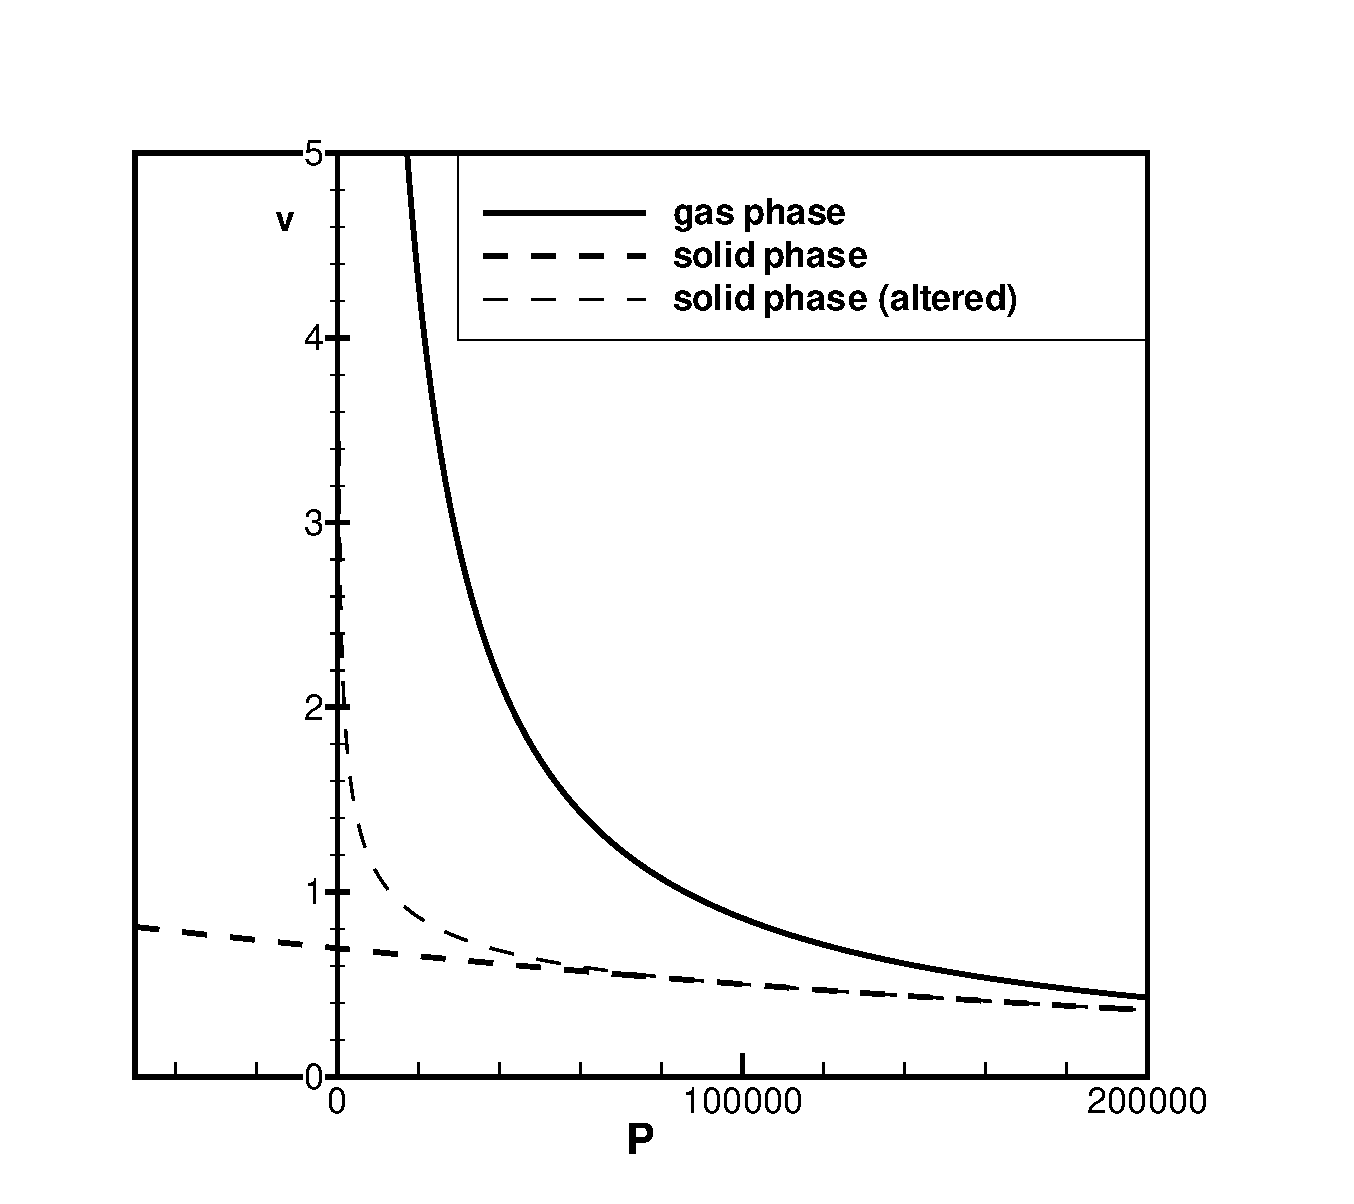
\includegraphics{Figs/mpmice/v_p_new.pdf}}
 \caption{Specific volume {\it vs} pressure for a gas phase material 
          and a solid phase material.  Light dashed line reflects an 
          altered solid phase equation of state to keep all materials
          in positive equilibration pressure space.}
 \label{vpfig}
\end{figure}

Recall that the isothermal compressiblity is the negative slope of
the specific volume versus pressure.  Embedded structures considered here are
solids and, at low pressure, possess a much smaller
compressibility than the gasses in which they are submerged.  
Nevertheless the variation of condensed phase specific volume can be important
at very high pressures, where the compressibilities of the gas and condensed
phase materials can become comparable (as in a detonation wave, for
example).  Because the speed of shock waves in materials is determined by
their equations of state, obtaining accurate high pressure behavior is an
important goal of our FSI studies.

To compensate for the lack of directional information for the embedded
surfaces, we evaluate the solid phase equations of state
in two parts.  Above a specified postive threshold pressure 
(typically 1 atmosphere), the full equation of state is respected; below that 
threshold pressure, the solid phase pressure follows a
polynomial chosen to be $C^1$ continuous at the threshold value and
which approaches zero as the specific volume becomes large.  The effect
is to decouple the solid phase specific volume from the stress
when the isotropic part of the stress falls below a threshold value.  In 
regions of coexistence at states below the threshold pressure, $p$ tends 
to behave according to the fluid equation of state (due to the greater 
compressibility) while in regions of pure condensed phase material $p$ tends 
rapidly toward zero and the full material stress dominates the dynamics as 
it should.

\subsection{The Material Point Method}\label{sec:mpm}

Solid materials with history dependent constitutive relations are more 
conveniently treated in the Lagrangian frame.  Here we briefly describe a 
particle method known as the Material Point Method (MPM) which is used to 
evolve the equations of motion for the solid phase materials.  MPM is a 
powerful technique for computational solid mechanics, and has found favor 
in applications involving complex geometries~\cite{Guilkey2006}, large 
deformations ~\cite{Brydon2005} and fracture~\cite{Guo2004}, to name 
a few.  After the description of MPM, its incorporation 
within the multi-material solution is described in 
Sec.~\ref{sec:coupling}.

Originally described by Sulsky, et al., \cite{Sulsky1994,Sulsky1995}, 
MPM is a particle method for structural mechanics simulations.  MPM is an 
extension to solid mechanics of FLIP \cite{brackbill-ruppel86}, which is a 
particle-in-cell (PIC) method for fluid flow simulation.  The method typically
uses a cartesian grid as a computational scratchpad for computing
spatial gradients.  This same grid also functions as an updated Lagrangian grid
that moves with the particles during advection and thus eliminates the
diffusion problems associated with advection on an Eulerian grid.  At the end
of a timestep, the grid is reset to the original, regularly ordered, position.

In explicit MPM, the equations of motion are cast in the form \cite{Sulsky1995}:
\begin{eqnarray}
        \Bm \Ba &=& \BF^{\rm{ext}} - \BF^{\rm{int}}  \label{newton2}
\end{eqnarray}
where $\Bm$ is the mass matrix, $\Ba$ is the acceleration vector,
$\BF^{\rm{ext}}$ is the external force vector (sum of the body forces and
tractions), and $\BF^{\rm{int}}$ is the internal force vector resulting from
the divergence of the material stresses.

The solution procedure begins by projecting the particle state to the
nodes of the computational grid, to form the mass matrix $\Bm$ and to find
the nodal external forces $\BF^{\rm{ext}}$, and velocities,
$\Bv$.  In practice, a lumped mass matrix is usually used.
These quantities are calculated at individual nodes by the following 
equations, where the $\sum\limits_{p}$ represents a summation over all 
particles:
\begin{eqnarray}
m_i = \sum_{p} S_{ip} m_p,  \;\;\;\;\;\; 
\Bv_i = \frac{\sum\limits_{p} S_{ip} m_p \Bv_p}{m_i},  \;\;\;\;\;\;
\BF^{\Text}_i &=& \sum_{p} S_{ip} \BF^{\Text}_p
\label{interpolate}
\end{eqnarray}
and $i$ refers to individual nodes of the grid.  $m_p$ is the particle
mass, $\Bv_p$ is the particle velocity, and $\BF^{\Text}_p$ is the external
force on the particle.
$S_{ip}$ is the $i$th node's shape function evaluated at the particle position $\Bx_p$.
Traditionally, standard tri-linear shape functions are used, but recently
smoother interpolants, as described in \cite{Bard2004}, have yielded
improved results.

A velocity gradient,  $\nabla \Bv_p$ is computed at
the particles using the velocities projected to the grid:
\begin{equation}
\nabla \Bv_p = \sum_i \BG_{ip} \Bv_i
\label{velgrad}
\end{equation}
where $\BG_{ip}$ is the gradient of the shape function of the $i$th node
evaluated at $\Bx_p$.

This is used as input to a constitutive model which is evaluated on a
per particle basis, the result of which is the Cauchy stress at each
particle, $\Bsig_p$.  With this, the internal force due to the divergence
of the stress is calculated via:
\begin{eqnarray}
        \BF^{\Tint}_i &=& \sum_{p} \BG_{ip} \Bsig_p V_p,
\end{eqnarray}
where $V_p$ is the particle volume.

Equation \ref{newton2} can then be solved for $\Ba$.
An explicit forward Euler method is used for the time integration:
\begin{eqnarray}
\Bv^L= \Bv + \Ba~\DelT
\label{MPM:euler}
\end{eqnarray}
and the particle position and velocity are explicitly updated by:
\begin{eqnarray}
  \Bv_p (t + \DelT)  &=& \Bv_p (t)  + \sum_{i} S_{ip} ~\Ba_i  ~\DelT 
  \label{MPM:updateVp} \\
  \Bx_p (t + \DelT)  &=& \Bx_p (t)  + \sum_{i} S_{ip} ~\Bv^L_i  ~\DelT 
  \label{MPM:updateXp}
\end{eqnarray}
This completes one timestep.

By describing and implementing MPM in an independent fashion, validation of 
the method itself as well as submodels (e.g., constitutive models and contact)
is simplified.  However, we emphasize that its use here is for selected 
material field description within the general multi-material formulation.  This 
integration is described next.

\subsection{Integration of MPM within the Eulerian Multi-Material 
            Formulation}\label{sec:coupling}

An important feature of this work is the ability to represent a material in 
either the Lagrangian or Eulerian frame.  This allows treating specific phases 
in their traditionally preferred frame of reference.
The Material Point Method, is used to time 
advance solid materials that are best described in a Lagrangian reference frame.
By choosing the background grid used to update the solid materials to
be the same grid used in the multi-material Eulerian description,
all interactions among materials can be computed in the common
framework, according to the momentum and heat exchange terms in 
Eqs~\ref{eqmomr}-\ref{eqenergyr}.  This results in a robust and tightly 
coupled solution for interacting materials with very different responses.

To illustrate how the integration is accomplished in an algorithmic fashion 
the explicit steps for advancing a fluid-structure interaction problem from 
time $t$ to time $t+\Delta{t}$ are described below.
\begin{enumerate}

%\setlength{\topsep=0.1in}
%\setlength{\itemsep=0.0in}
%\setlength{\parskip=0.1in}
%\setlength{\partopsep=0.4in}

\item {\bf Project particle state to grid:} A simulation timestep begins by
interpolating the particle description of the solid to the grid.  This starts
with a projection of particle data to grid vertices, or nodes, as described
in Eq.~\ref{interpolate}, and is followed by a subsequent projection from
the nodes to the cell-centers.  Since our work uses a uniform structured
grid, each node has equal weight in its contribution to the cell-centered
value.  The exception to this is near computational boundaries where
symmetric boundary conditions are used.  The weight of those nodes on
the boundary must be doubled in order to achieve the desired effect.

\item {\bf Compute the equilibrium pressure:} While Eq.~\ref{mmeos} and the
surrounding discussion describes the basic process, one specific point warrants
further explanation.  In particular, the manner in which each material's
volume fraction is computed is crucial.  Because the solid and fluid materials 
are evolved in different frames of reference, the total volume of material in a 
cell is not necessarily equal to the volume of a computational cell.  Material 
volume is tracked by evolving the specific volume for each material 
according to Eq.~\ref{eqspvolr}.
The details of this are further described in step 11.

With the materials' masses and specific volumes, material volume
can be computed ($V_r=M_r v_r$) and summed to find the total material volume.  The volume
fraction $\theta_r$ is then computed as the volume of r-material per total
material volume.  With this, the solution of Eq.~\ref{mmeos} can be carried
out at each cell using a Newton-Raphson technique\cite{Harlow1975},
which results in new values for the equilibrium pressure, $p_{\Teq}$,
volume fraction, $\theta_r$ and specific volume, $v_r$.

\item {\bf Compute face-centered velocities, $u^*_r$, for the 
           Eulerian advection:}
At this point, fluxing velocities are computed at each cell face.  The 
expression for this is based on a time advanced estimate for the cell-centered 
velocity.  A full development can be found in  \cite{Kashiwa1994a} and 
\cite{Kashiwa2000} but here, only the result is given:
\begin{equation}
u^*_r = \frac{\rho_{r_L} u_{r_L} + \rho_{r_R} u_{r_R}}
                {\rho_{r_L} + \rho_{r_R}} -
           \left( \frac{2 v_{r_L} v_{r_R} \Delta{t}}
                       {v_{r_L} + v_{r_R}}\right)
           \left( \frac{p_{{\Teq}_R} - p_{{\Teq}_L}}{\Delta{x}}\right) + g\Delta{t}
\end{equation}
The first term above is a mass weighted average of the logically left and right
cell-centered velocities, the second is a pressure gradient acceleration
term, and the third is acceleration due to the component of gravity in the face 
normal direction.  Not shown explicitly is the necessary momentum exchange at the
face-centers.  This is done on the faces in the same manner as described subsequently
in step 10 for the cell-centered momentum exchange.

\item {\bf Multiphase chemistry:} Compute sources of mass, momentum, energy
and specific volume as a result of phase changing chemical reactions for 
each r-material, $\Gamma_r$, $u_r \Gamma_r$, $e_r \Gamma_r$,
and $v_r \Gamma_r$.  Specifics of the calculation of $\Gamma_r$ are 
model dependent, and examples are given in Sec.~\ref{sec:HEReaction}.

Care must be taken to reduce the momentum, internal energy and volume of the 
reactant by an amount proportional to the mass consumed each timestep, so that 
those quantities are depleted at the same rate as the mass.  When the reactant 
material is described by particles, decrementing
the particle mass automatically decreases the momentum and internal energy
of that particle by the appropriate amount. This mass, momentum, 
and internal energy is transferred to the product material's state, 
and the volume fraction for the reactant and product materials is recomputed.

\item {\bf Compute an estimate of the time advanced pressure, $p$:}  Based on
the volume of material being added to (or subtracted from) a cell in a given 
timestep, an increment to the cell-centered pressure is computed using:

\begin{eqnarray}
     \Delta p &=&
     \DelT~ \frac{ \sum\limits_{r=1}^N v_r\Gamma_r
    -\sum\limits_{r=1}^N \nabla \cdot (\theta^{*}_r {u}^{*}_r)}
     {\sum\limits_{r=1}^N \theta_r\kappa_r}
    \label{eq:delP} \\
    p&=&p_{\Teq}+\Delta p \label{eq:time_adv_press}
\end{eqnarray}
where $\kappa_r$ is the r-material bulk compressibility.  The first term in 
the numerator of Eq.~\ref{eq:delP} represents the change in volume due to 
reaction, i.e., a given amount of mass would tend to occupy more volume in 
the gas phase than the solid phase, leading to an increase in pressure.  The 
second term in the numerator represents the net change in volume of material 
in a cell due to flow into or out of the cell.  The denominator is essentially 
the mean compressibility of the mixture of materials within that cell.  
This increment in pressure 
is added to the equilibrium pressure computed in step 2 and is the pressure 
used for the remainder of the current timestep.  Again, the details leading
to this equation can be found in \cite{Kashiwa1994a}.

\item {\bf Face Centered Pressure $p^*$:}
The calculation of $p^*$ is discussed at length in \cite{Kashiwa2000}.
For this work, it is computed using the updated pressure by:
\begin{equation}
p^* = {\left (\frac{p_L}{\rho_L} + \frac{ p_R}{\rho_R}\right)}/
                     {\left (\frac{1}{\rho_L} + \frac{1}{\rho_R}\right)}
\end{equation}
where the subscripts $L$ and $R$ refer to the logically left and right 
cell-centered values, respectively, and $\rho$ is the sum of all material's 
densities in that cell.  This will be used subsequently for the computation 
of the pressure gradient, $\nabla{ p^*}$.

\item {\bf Material Stresses:} For the solid, we calculate the velocity
gradient at each particle based on the grid velocity (Eq.~\ref{velgrad}) for use
in a constitutive model to compute particle stress.  Fluid stresses are
computed on cell faces based on cell-centered velocities.

\item {\bf Accumulate sources of mass, momentum and energy at cell-centers:}
These terms are of the form:
\begin{eqnarray}
%mass
 \Delta(m)_r &=& \DelT~ V \sum\limits_{s=1, s\ne r}^N \Gamma_s 
   \label{deltamass}\\
 %momentum
 \Delta(mu)_r &=& -\DelT~ V \left[\theta_r\nabla{ p^*} 
 + \nabla{ \cdot \theta_r (\Bsig_r - \Bsig) }
 + \sum_{s=1, s\ne r}^N u_s \Gamma_s\right] \label{deltamom} \\
 %energy
 \Delta(me)_r &=&  -\DelT~ V \left[\fthetar p
     \sum\limits_{s=1}^N \nabla \cdot (\theta^{*}_r {u}^{*}_r)
 + \sum\limits_{s=1, s\ne r}^N e_s \Gamma_s \right] \label{deltenergy}
 \end{eqnarray}
Note that the only source of internal energy
being considered here is that due to ``flow work".  This is required 
for the compressible flow formulation, but other terms, such as heat 
conduction are at times included.

\item {\bf Compute Lagrangian phase quantities at cell-centers:} The
increments in mass, momentum and energy computed above are added
to their time $t$ counterparts to get the Lagrangian values for these 
quantities.
Note that here, some Lagrangian quantities are denoted by an $L-$ superscript.
This indicates that all physical processes have been accounted for except for
inter-material exchange of momentum and heat which is described in the following step.

 \begin{eqnarray}
 (m)_r^L &=& (m)_r^t + \Delta(m)_r \label{lagmass} \\
 (m u)_r^{L-} &=& (mu)_r^t + \Delta(mu)_r \label{lagmom} \\
 (m e)_r^{L-} &=& (m e)_r^t + \Delta(m e)_r \label{lagenergy}
\end{eqnarray}

\item {\bf Momentum and heat exchange:} The exchange of momentum and heat 
between materials is computed according to:
\begin{eqnarray}
(m u)_r^L &=& (m u)_r^{L-} +
  \DelT~ m_r 
  \sum\limits_{s=1}^N \theta_r\theta_s K_{rs}(u_s^L - u_r^L) 
  \label{eqmomex} \\
(m e)_r^L &=& (m e)_r^{L-}+ 
  \DelT~m_r~ c_{v_r} 
  \sum\limits_{s=1}^N \theta_r 
     \theta_s H_{rs}\left(T_s^L - T_r^L \right) \label{eqheatex}
\end{eqnarray}
These equations are solved in a pointwise implicit manner that allows 
arbitrarily large momentum transfer to take place between materials.  Typically,
in FSI solutions, very large ($10^{15}$) values of $K$ are used, which results
in driving contacting materials to the same velocity.  Intermaterial heat
exchange is usually modeled at a lower rate.  Again, note that the same 
operation must be done following Step 3 above in the computation of the 
face-centered velocities.

\item {\bf Specific volume evolution:} As discussed above in step 2, in order to
correctly compute the equilibrium pressure and the volume fraction, it is necessary
to keep an accurate accounting of the specific volume for each material.  Here, 
we compute the evolution in specific volume due to the changes in temperature 
and pressure, as well as phase change, during the foregoing Lagrangian 
portion of the calculation, according to:
\begin{eqnarray}
  \Delta(mv)_r &=& \DelT~ V 
     \left[ v_r \Gamma_r 
        + \fthetar \nabla \cdot \sum\limits_{s=1}^N{\theta_s^*u_s^*}
               + \theta_r \beta_r \dot{T_r} 
        - \fthetar \sum\limits_{s=1}^N{\theta_s \beta_s \dot{T_s}}\right]   
     \label{eqspvoldiscrete} \\
  (mv)_r^L &=& (mv)_r^n + \Delta(mv)_r \label{eqspvolLag}
\end{eqnarray}
where $\beta$ is the constant pressure thermal expansivity and
$\dot{T}=\frac{T^L - T^t}{\Delta{t}}$ is the rate of change of each material's
temperature during the Lagrangian phase of the computation.

\item {\bf Advect Fluids:} For the fluid phase, use a suitable advection scheme,
such as that described in \cite{Kashiwa1998}, to transport mass, momentum, internal energy 
and specific volume.  As this last item is an intensive quantity, it is converted
to material volume for advection, and then reconstituted as specific volume
for use in the subsequent timestep's equilibrium pressure calculation.

\item{\bf Update Nodal Quantities for Solid Materials:}  Those changes in 
solid material mass, momentum and internal energy that are computed at the 
cell-centers are interpolated to the nodes as field quantities, e.g., changes 
in momentum are expressed as accelerations, for use in Eq.~\ref{MPM:euler}.

\item {\bf Advect Solids:} For the solid phase, interpolate the time advanced
grid velocity and the corresponding velocity increment (acceleration) back 
to the particles, and use these to advance the particle's position and 
velocity, according to Eqs.~\ref{MPM:updateVp}-\ref{MPM:updateXp}.

\end{enumerate}

This completes one timestep.  In the preceding, the user has a number of
options in the implementation.  The approach taken here was to develop a 
working MPM code and a separate working multi-material ICE code.  In 
addition, some routines specific to the integration are required, for 
example, to transfer data from grid nodes to cell-centers.  We 
note, however, that the fluid structure interaction methodology should 
not be looked at in the context of a ``marriage" between an Eulerian CFD 
code and MPM.  The underlying theory is a multi-material description
that has the flexibility to incorporate different numerical descriptions for 
solid and fluid fields within the overarching solution process. 
To have flexibility in treating a widest range of problems, it was our 
desire that in the integration of the two algorithms, each of the components 
be able to function independently.  As described here, this method is fully 
explicit in time.  To make this implicit with respect to the propagation 
of pressure waves, a Poisson equation is solved in the calculation of 
$\Delta p$, which is in turn used to iteratively update the face-centered 
velocities \cite{Kashiwa1994a}.

\section{Models}\label{sec:models}

The governing equations given in Section~\ref{sec:governing_equations} are 
incomplete without closure equations for quantities such as pressure, stress, 
and rate of exchange of mass between materials.  Equations of 
state, constitutive models and reaction models provide
the needed closure.  Brief descriptions of some of the models used in this work 
are given below.

\subsection{High Energy Material Reaction Models}\label{sec:HEReaction}

Two types of High Energy (HE) reaction models were considered here.  The first 
is a model for detonation, in which the reaction front proceeds as a shock 
wave through the solid reactant, leaving highly pressurized product gases 
behind the shock.  The second is a deflagration model, in which the 
reaction proceeds more slowly through the reactant in the form of a thermal
burn.  Each is described here.

\subsubsection{The JWL++ Detonation Model}\label{sec:JWLPP}

The detonation model used in two of the calculations discussed in 
Section~\ref{sec:numerical_results} is a reactive flow model known as 
JWL++\cite{JWLpp}.  JWL++ consists of equations of state for the
reactant and the products of reaction as well as a rate equation governing 
the transformation from product to reactant.  In addition, the model consists 
of a ``mixer" which is a rule for determining the pressure in a mixture of 
product and reactant, as found in a partially reacted cell.  Because pressure 
equilibration among materials is already part of the  multi-material CFD 
formulation described in Section~\ref{sec:numerical_algorithm}, the mixer was 
not part of the current implementation.  Lastly, two additional rules 
apply.  The first is that reaction begins in a cell when the pressure in that
cell exceeds 200 MPa.  Finally, no more than 20\% of the explosive in a cell 
is allowed to react in a given timestep.

The Murnaghan equation of state~\cite{Murnaghan1944} used for the solid reactant 
material is given by:
\begin{eqnarray}
p=&{1\over n \kappa}\left({1\over v^n}-1\right)&
\label{Murnaghan}
\end{eqnarray}
where $v=\rho_0/\rho$, and $n$ and $\kappa$ are material dependent model 
parameters.  Note that while the reactants are solid materials, they are 
assumed to not support deviatoric stress.  Since a detonation propagates 
faster than shear waves, the strength in shear of the reactants can be 
neglected.  Since it is not necessary to track the deformation history 
of a particular material element, in this case, the reactant material was 
tracked only in the Eulerian frame, \textit{i.e.} not represented by 
particles within MPM.

The JWL C-term form is the equation of state used for products, and is 
given by:
\begin{eqnarray}
P=&A \exp(-R_1 v) + B \exp(-R_2 v) + {C\over {\rho_0 \kappa v^{n-1}}}&
\label{JWLC}
\end{eqnarray}
where $A$, $B$, $C$, $R_1$, $R_2$, $\rho_0$ and $\kappa$ are all 
material dependent model parameters.

The rate equation governing the transformation of reactant to product is 
given by:
\begin{eqnarray}
{dF \over dt}=&G(p+q)^b(1-F)
\label{JWL++rate}
\end{eqnarray}
where $G$ is a rate constant, and 
$b$ indicates the power dependence on pressure.  $q$ is an artificial 
viscosity, but was not included in the current implementation of
the model.  Lastly:
\begin{eqnarray}
F={{\rho_{\Tproduct}}\over{\rho_{\Treactant}+\rho_{\Tproduct}}}
\end{eqnarray}
is the burn fraction in a cell.  This can be differentiated and solved for 
a mass burn rate in terms of $dF$:

\begin{eqnarray}
\Gamma&=&{dF \over dt}  \left(\rho_{\Treactant}+\rho_{\Tproduct}\right)
\end{eqnarray}

\subsubsection{Deflagration Model}\label{sec:deflagration}

The rate of thermal burning, or deflagration, of a monopropellant 
solid explosive is typically assumed to behave as:

\begin{eqnarray}
D&=&Ap^n
\label{deflagration_rate}
\end{eqnarray}
where $D$ can be thought of as the velocity at which the burn front 
propagates through the reactant (with units of length/time) and $p$ is the 
local pressure~\cite{Son2000}.  $A$ and $n$ are parameters that are 
empirically determined for particular explosives.  
Because deflagration is a 
surface phenomenon, our implementation requires the identification of the 
surface of the explosive.  The surface is assumed to lie within those cells 
which have the highest gradient of mass density of the reactant 
material.  Within each surface cell, an estimate of the surface area $a$
is made based on the direction of the gradient, and the rate $D$ above 
is converted to a mass burn rate by:
\begin{eqnarray}
\Gamma&=&a D \rho_{\Treactant}
\label{deflagration_mass_rate}
\end{eqnarray}
where $\rho_{\Treactant}$ is the local density of the explosive.  While the reaction 
rate is independent of temperature, initiation of the burn depends 
on reaching a threshold temperature at the surface.

Since the rate at which a deflagration propagates is much slower than the 
shear wave speed in the reactant, it is important to track its deformation 
as pressure builds up within the container.  This deformation may lead to 
the formation of more surface area upon which the reaction can take place, and 
the change to the shape of the explosive can affect the eventual violence of the
explosion.  Because of this, for deflagration cases, the explosive is 
represented by particles in the Lagrangian frame.  The stress response is 
treated by an implementation of ViscoSCRAM \cite{Hackett2000Viscoscram}, which includes 
representation of the material's viscoelastic response, and considers effects 
of micro-crack growth within the granular composite material.

\subsection{Constitutive Model for Container Breakup}\label{sec:cons_mod}

  One of the unique features of the approach described here is its ability to 
  treat the interaction of fluid regions that are initially separated by a 
  solid material.  Such a situation is found when gaseous products of 
  reaction are contained in a metal canister surrounded by air.  When the 
  pressure within the container is sufficient, it will rupture and the 
  product material will be in direct contact with the surrounding air.  Given 
  the ability to treat these situations, it is worthwhile to accurately 
  describe the failure of the container.

  While a full exposition of metal  
  plasticity and failure is beyond the scope of this manuscript, a brief 
  description of the current implementation is given here.  More details of
  the models and algorithms can be found elsewhere 
  ~\cite{Banerjee2005,Banerjee2005b,Banerjee2005d}.

  The metal container is modeled as a
  hypoelastic-plastic material.  The Green-Naghdi stress rate is used to 
  provide objectivity to the constitutive equation.  The Cauchy stress is 
  additively decomposed into a volumetric component and a deviatoric 
  component.  

  The volumetric stress is computed using a Mie-Gr{\"u}neisen equation of 
  state~\cite{Zocher2000}:
  \begin{equation} \label{eq:EOSMG}
   p = \frac{\rho_0 C_0^2 (\eta -1)
              \left[\eta - \frac{\Gamma_0}{2}(\eta-1)\right]}
             {\left[\eta - S_{\alpha}(\eta-1)\right]^2} + \Gamma_0 E~;~~
   \eta = \rho/\rho_0
  \end{equation}
  where $p$ is the pressure, $C_0$ is the bulk speed of sound,
  $\Gamma_0$ is the Gr{\"u}neisen's gamma at the reference state,
  $S_{\alpha}$ is a linear Hugoniot slope coefficient,
  $E$ is the internal energy per unit reference specific volume,
  $\rho_0$ is the initial density, and $\rho$ is the current density, 

 In the elastic domain, the deviatoric stress is computed using 
  a hypoelastic model with a constant shear modulus.  The von Mises yield 
  condition is used to determine whether the material is in the plastic 
  domain.  The flow stress ($\sigma_y$) is computed using the Johnson-Cook
  model~\cite{Johnson1983}: 
  \begin{align}
    \sigma_y(\Ep,\Epdot{},T) & =
    \sigma_0\left[1 + \cfrac{B}{\sigma_0} (\Ep)^n\right]
            \left[1 + C \ln(\Epdot{}^{*})\right]
            \left[1 - (T^*)^m\right] \\
    \Epdot{}^{*} & = \cfrac{\Epdot{}}{\Epdot{0}}; \quad
    T^* = \cfrac{(T-T_0)}{(T_m-T_0)}
  \end{align}
  where $\sigma_0$ is the yield stress at zero plastic strain, and
  $(B, C, n, m)$ are material constants, $\Ep$ is the equivalent plastic strain,
  $\Epdot{}$ is the plastic strain rate, $\Epdot{0}$ is a reference strain
  rate, $T_0$ is a reference temperature, and $T_m$ is the melt temperature.
  
  The plastic strain and the deviatoric Cauchy stress in the plastic domain 
  are computed with a semi-implicit stress update 
  algorithm~\cite{Nemat1991,Maudlin1996}.  A portion of the plastic work is
  converted into heat using a Taylor-Quinney coefficient of 0.9.  The 
  temperature of a material point is updated accordingly.
  
  Experiments show that metal containers fail both by void nucleation and growth
  and by adiabatic shear banding.  We use three criteria to determine whether a
  material point has failed.
  
  \begin{enumerate}
    \item {
       {\bf Melting:}\hspace{12pt}  
       A material point is tagged as "failed" when its 
       temperature is greater than the melting point of the material at the 
       applied pressure.  
       \vspace{10pt}
       }

    \item {
       {\bf TEPLA-F failure condition:} \hspace{12pt}
       A material point is also assumed
       to have failed when the TEPLA-F failure criterion~\cite{Johnson1988} 
       is satisfied.  This criterion can be written as
       \begin{equation}
         (f/f_c)^2 + (\Ep/\Ep^f)^2 = 1
       \end{equation}
       where $f$ is the current porosity, $f_c$ is the maximum 
       allowable porosity, $\Ep$ is the current plastic strain, and
       $\Ep^f$ is the plastic strain at fracture.

       The evolution of porosity is given by~\cite{Chu1980,Ramaswamy1998a}: 
       \begin{align}
         \dot{f} &= \dot{f}_{\text{nucl}} + \dot{f}_{\text{grow}} \\
         \dot{f}_{\text{grow}} & = (1-f) \text{tr}(\BD_p) \\
         \dot{f}_{\text{nucl}} & = \cfrac{f_n}{(s_n \sqrt{2\pi})}
           \exp\left[-\Half \cfrac{(\Ep - \epsilon_n)^2}{s_n^2}\right]
           \Epdot{}
       \end{align}
       where $\BD_p$ is the rate of plastic deformation tensor, $f_n$ is the 
       volume fraction of void nucleating particles , $\epsilon_n$ is the mean 
       of the distribution of nucleation strains, and $s_n$ is the standard 
       deviation of the distribution.  A gaussian distribution of initial 
       porosity is assumed.

       The plastic strain at fracture is determined using the Johnson-Cook
       damage model~\cite{Johnson1985}:
       \begin{equation}
         \Ep^f = 
         \left[D_1 + D_2 \exp \left(\cfrac{D_3}{3} \sigma^*\right)\right]
         \left[1+ D_4 \ln(\dot{\epsilon_p}^*)\right]
         \left[1+D_5 T^*\right]~;~~
         \sigma^*= \cfrac{\text{tr}(\Bsig)}{\sigma_{eq}}~;~~
       \end{equation}
       where $D_1, D_2, D_3, D_4, D_5$ are material constants, 
       $\Bsig$ is the Cauchy stress, and $T^*$ is the homologous temperature.
       We assume that the plastic strains at failure are also distributed
       in a gaussian manner.  The distribution of fracture strains is 
       simulated by evolving an internal damage variable based on the plastic 
       strain and by initializing the damage variable to a non-zero value
       at the beginning of the simulation.
       \vspace{10pt}
       }

    \item {
       {\bf Loss of material stability:} \hspace{12pt}
       The third criterion that is used to 
       determine failure is the loss of material stability of the solid.
       Since this condition is not sufficient to determine failure, we check
       two conditions - the Drucker stability condition~\cite{Drucker1959} 
       and the loss of hyperbolicity of the governing equations (the determinant
       of the acoustic tensor changes sign)~\cite{Rudnicki1975,Perzyna1998}.  

       Determination of the acoustic tensor requires a search for a normal 
       vector around the material point and is therefore computationally 
       expensive.  A simplification of this criterion is a check which 
       assumes that the direction of instability lies in the plane of the 
       maximum and minimum principal stress~\cite{Becker2002}.  In this 
       approach, we assume that the strain is localized in a band with 
       normal $\Bn$, and the magnitude of the velocity difference across 
       the band is $\Bg$.  Then the bifurcation condition leads to the relation 
       \begin{equation} 
         R_{ij} g_{j} = 0 ~;~~~
         R_{ij} = M_{ikjl} n_k n_l + M_{ilkj} n_k n_l - \sigma_{ik} n_j n_k
       \end{equation} 
       where $M_{ijkl}$ are the components of the co-rotational tangent
       modulus tensor and $\sigma_{ij}$ are the components of the co-rotational 
       stress tensor.  If $\det(R_{ij}) \le 0 $, then $g_j$ can be arbitrary 
       and there is a possibility of strain localization.  

       If this condition 
       for the loss of hyperbolicity is met, a material point deforms in an 
       unstable manner and failure is assumed to have occurred at that point.  
       }
  \end{enumerate}
  
  After it has been determined that a material point has failed, the stress
  at that point is set to zero - indicating that a free surface has been 
  created.  As the simulation evolves, cracks develop in the material around
  the failed particles ultimately leading to the break-up of the container.
  
 
\section{Numerical Results}\label{sec:numerical_results}

  The simulation results presented here are intended to serve two purposes, to 
  validate the method presented above, and to demonstrate its 
  capabilities.  While results from some very basic validation tests can be 
  found in \cite{Guilkey2005}, the validation tests presented here are 
  targeted toward exploding energetic devices.  Extensive experimental data have
  been collected for the first two cases, and these data are compared with 
  simulation results.  
  
  The first test, detonation of a series of cylinders of explosive, validates 
  both the general multi-material framework, including material 
  transformation, as well as the detonation model itself.  In the second 
  test, a cylinder of explosive confined in a copper tube is 
  detonated.  There, the confidence gained from the 
  first test is built upon and extended to include the interaction of the highly
  pressurized product gases with the confining copper cylinder.  Wall velocity 
  of the copper tube is compared with experimental measurements.

  For the last case, a steel cylinder filled with PBX-9501 is heated to the 
  critical temperature to commence a deflagration.  The simulation continues 
  through the rupture of the case when product gases are 
  free to interact with the surrounding air.  This simulation demonstrates a 
  unique capability of this approach, in which initially separate fluid 
  regions are allowed to interact following the failure of the steel container.

\subsection{Rate Stick Simulations}

A well known phenomenon of detonating solid high explosives is the 
so-called ``size effect".  The size effect refers to the change of the 
steady state detonation velocity of explosives, $U_s$ with size $R_0$
\cite{JWLpp}.  In order to validate our implementation of the JWL++ 
detonation model within our multi-material framework, a parameter study 
was conducted for cylinders of Ammonium Nitrate Fuel Oil (ANFO-K1) with 
length of 10 cm and radii ranging from 4 mm to 20 mm.  In addition, a 
one-dimensional simulation provided for the ``infinite radius" case.  In each of the finite radius 
cases, the cylinder was initially surrounded by air.  Detonation was 
initiated by impacting the cylinder at 90 m/s against the boundary of the 
computational domain, at which a zero velocity Dirichlet boundary condition 
was imposed.  This impact was sufficient to raise the pressure within the 
cylinder to above the threshold for initiation of reaction.  The detonation 
velocity was determined by comparing the arrival time of the detonation at 
two points along the cylinder, sufficiently into the far field that the
detonation had reached a steady state.

Material properties for these cases included the following:  The reactant was 
described by a Murnaghan equation of state with parameters $n$ = 7.4, 
$\kappa$ = 3.9$\times$10$^{11}$ Pa$^-1$ and $\rho_0$ = 1160.0 kg/m$^3$.  The products of 
reaction were described by a JWL C-term form  equation of state with parameters
$A$ = 2.9867$\times$10$^{11}$ Pa, $B$ = 4.11706$\times$10$^9$ Pa, $C$ = 7.206147$\times$10$^8$ Pa, $R_1$ = 4.95, 
$R_2$ = 1.15, $\omega$ = 0.35 and $\rho_0$ = 1160.0 kg/m$^3$.  The JWL++ parameters 
were taken as: $G$ = 3.5083$\times$10$^{-7}$ s$^{-1}$Pa$^b$, $b$ = 1.3, $\rho_0$ = 1160.0 kg/m$^3$.  
In all, this simulation included 3 materials; the reactant material, the 
products of reaction and the surrounding air.

Simulations were carried out on uniform meshes with cell sizes of 1.0 mm, 
0.5 mm and 0.25 mm.  A one-quarter symmetry was assumed in all cases.  A 
qualitative representation is shown in Figure \ref{figRSVR}, which depicts a 
volume rendering of the density of the reactant as the detonation has progressed
about halfway into the material for the 12 mm radius case at the finest 
resolution.  The curvature of the burn front and the elevated density just 
ahead of it are evident in this view.

\begin{figure}
  \center
  \scalebox{0.5}{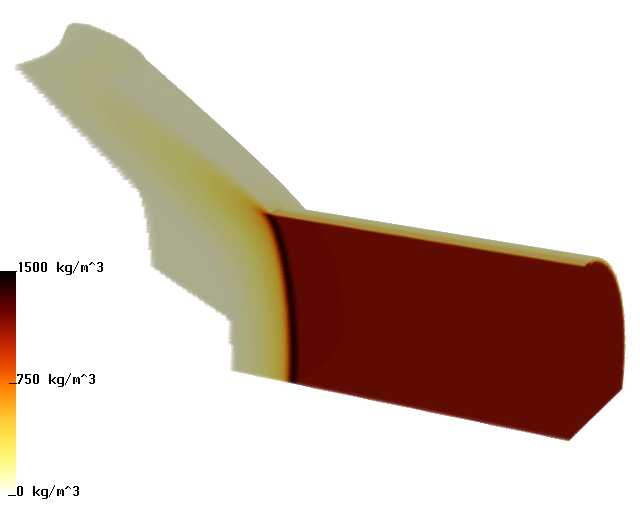
\includegraphics{Figs/mpmice/12mmRSVolRen.png}}
  \caption{Unconfined 12 mm ``rate-stick".  The mass density of the reactant 
           material is volume rendered, and shows evidence of the curvature 
           of the reaction front, and the compression of the reactant just 
           ahead of the reaction.  Behind the detonation, most of the reactant 
           material is consumed. }
  \label{figRSVR}
\end{figure}

Figure \ref{figRSSE} is  a plot of detonation velocity {\it{versus}} the inverse of 
the sample radius.  Experimental data are represented by open squares, 
while results of the simulations are shown with filled circles (h = 1.0 mm), filled
diamonds (h = 0.5 mm) and filled triangles (h = 0.25 mm).  Connecting lines for 
the numerical data are in place to guide the eyes of the reader.  Evident 
from this plot is the convergence of detonation velocities with grid 
resolution, and the generally good agreement between experimental and
computed detonation velocities at the finer grid resolutions, particularly 
at the larger radii, where both the experimental data and the model are 
considered more reliable.

\begin{figure}
  \center
  \scalebox{0.5}{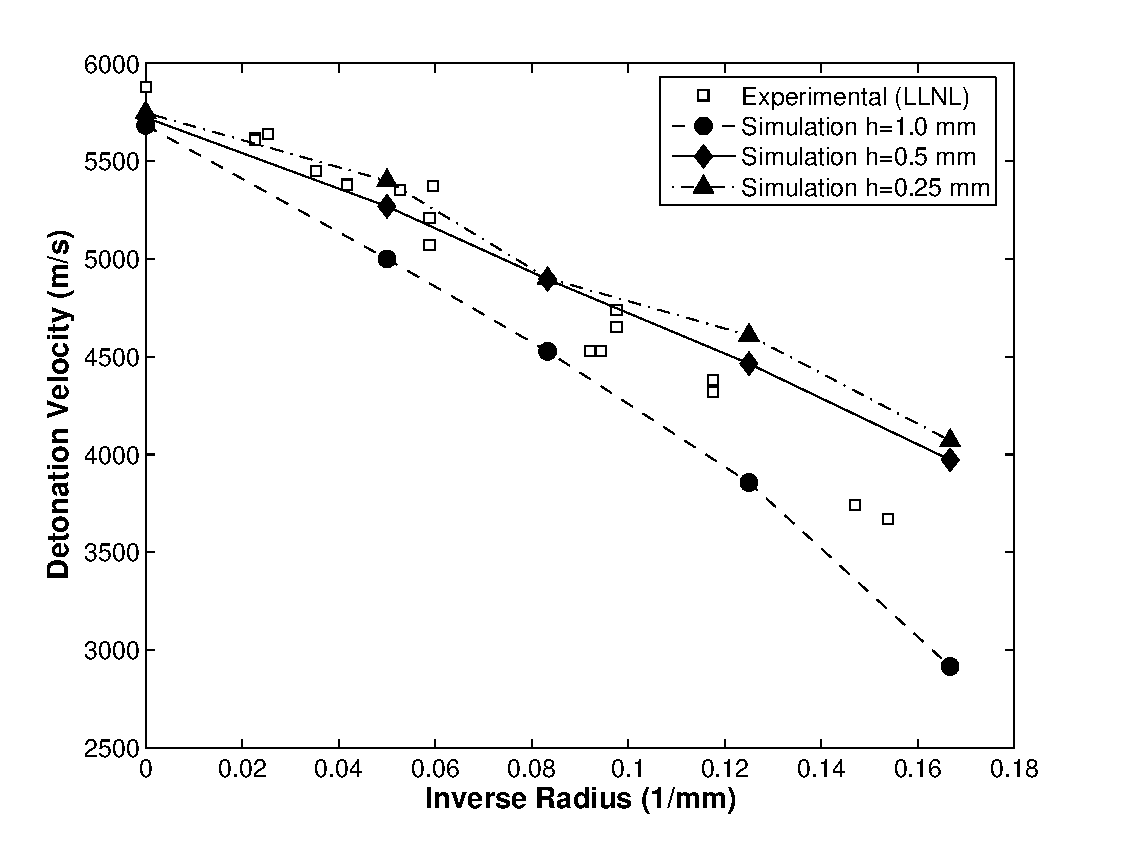
\includegraphics{Figs/mpmice/RateStick.pdf}}
  \caption{Detonation velocity vs. inverse radius.  Experimental and numerical 
          data are presented, and indicate good agreement of the model 
          with experiment, as well as convergence of detonation velocity 
          with grid resolution.}
  \label{figRSSE}
\end{figure}

Again, while this set of tests doesn't validate the full fluid-structure 
interaction approach, it does give credibility to the underlying 
multi-material formulation, including the pressure equilibration and the
exchange of mass between materials, in this case as governed by the 
JWL++ detonation model, as well as momentum and energy.

\subsection{Cylinder Test Simulation}

The cylinder test is an experiment which is frequently used to calibrate 
equations of state for detonation products of 
reaction~\cite{Souers2001CylinderTest}.  In this case, the test consists of an OFHC
copper tube with an inner radius of 2.54 cm, an outer radius of 3.06 cm and 
a length of 35 cm.  The tube is filled with QM-100, an Ammonium Nitrate 
emulsion and a detonation is initiated at one end of the tube.  Measurements
of the wall velocity wall are made at individual points along the length of 
the tube using Fabry-Perot interferometry or streak cameras.

A simulation of this configuration was performed and wall velocity data were 
collected at an axial location 25 cm from the point of initiation.  The 
reactant was again described by a Murnaghan equation of state with parameters 
$n$ = 7.0, $\kappa$ = 1.02$\times$10$^{-9}$ Pa$^{-1}$ and $\rho_0$ = 1260.0 kg/m$^3$.  The products 
of reaction were described by a JWL C-term form  equation of state with 
parameters $A$ = 4.8702$\times$10$^{11}$ Pa, $B$ = 2.54887$\times$10$^9$ Pa, $C$ = 5.06568$\times$10$^8$ Pa, 
$R_1$ = 5.0, $R_2$ = 1.0, $\omega$ = 0.3 and $\rho_0$ = 1260.0 kg/m$^3$.
The JWL++ parameters were taken as: $G$ = 9.1$\times$10$^{-5}$s$^{-1}$ Pa, $b$ = 1.0,
$\rho_0$ = 1260.0 kg/m$^3$.  The copper tube was modeled as an elastic-perfectly 
plastic material with a density of 8930.0 kg/m$^3$, bulk and shear moduli of 
117.0 GPa and 43.8 GPa, respectively,and a yield stress of 70.0 MPa.
The copper tube was surrounded by air.  In all, 4 materials are present in
this simulation, the reactant, the products of reaction, the copper tube, and 
the surrounding air.

Again, a one-quarter symmetry section of the full cylinder was modeled using 
a cell size of h = 0.5 mm and a total domain size of 
35 cm $\times$ 6 cm $\times$ 6 cm.  Zero gradient conditions described the 
exterior boundaries, which allowed material to exit the domain.

Figure \ref{figCuRSiso} shows a snapshot of this test midway through the 
simulation, at t = 18.8 $\mu$s.  The copper tube is depicted using an 
iso-surface of the cell-centered mass density (the two surfaces are the 
inner and outer walls of the tube) that is colored by velocity.  A volume 
rendering of the pressure field is also present.  Alternating bands of high 
and low velocity of the tube wall are evidently due to the reflection of the 
impulse provided by the shock between the inner and outer surfaces of the tube.

\begin{figure}
  \center
  \scalebox{0.5}{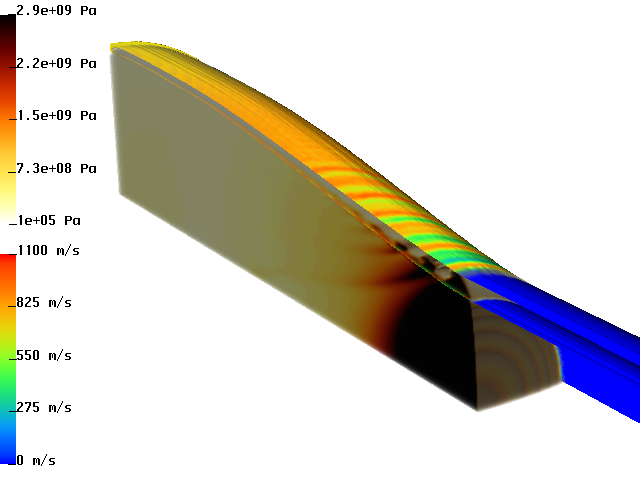
\includegraphics{Figs/mpmice/CuRS1.png}}
  \caption{Copper cylinder test simulation.  The walls of the copper tube 
           are depicted as an isosurface of density of the copper material 
           and are colored by velocity magnitude.  Pressure is represented by a
           volume rendering, and indicates the progress of the detonation, as 
           well as the interaction of the pressurized products of reaction 
           with the confining walls. }
  \label{figCuRSiso}
\end{figure}

Velocity data was collected from those particles which were both initially 
at an axial location of 25 cm, and upon the exterior surface of the tube.  The 
velocity from this collection of particles was averaged over the circumference 
and plotted vs. time in Figure \ref{figCuRSwallvel}.  In addition, experimental 
results (LLNL, Shot No. K260-581) are also shown.  Both datasets are time 
shifted to coincide with the arrival of the detonation.  Good agreement is 
evident between the experimental and numerical data, further indicating the 
validity of the approach described here.

\begin{figure}
  \center
  \scalebox{0.5}{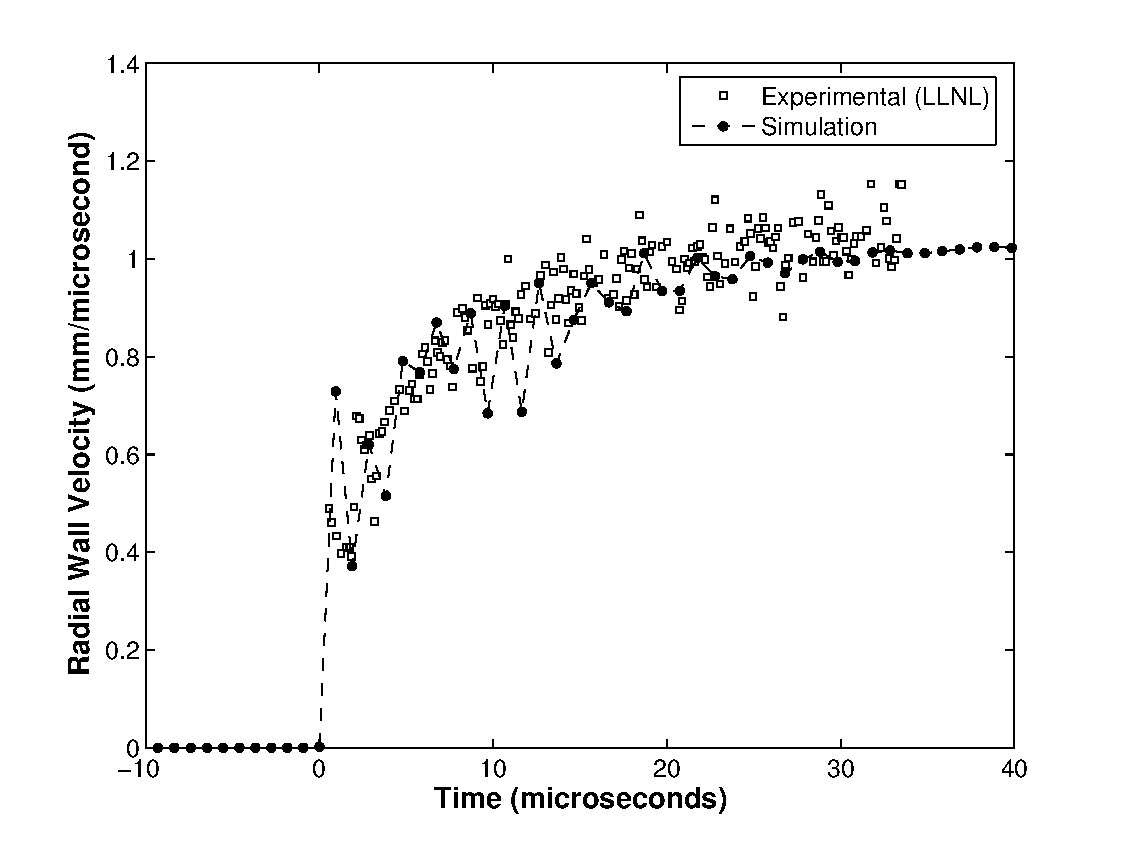
\includegraphics{Figs/mpmice/CuTubeWallVel.pdf}}
  \caption{Copper cylinder test simulation.  Experimental and computational 
           velocities of the cylinder vs. time. Data was collected at a 
           point 25 cm from the point of initiation of the detonation. }
  \label{figCuRSwallvel}
\end{figure}

\subsection{Fast Cookoff Simulation}

Cookoff tests, generally speaking, refer to experiments in which
energetic material is heated until it reaches ignition.  The rate of
heating typically differentiates these tests in to ``fast" or ``slow"
cookoff.  In slow cookoff tests, the temperature is usually increased
very slowly, perhaps a few degrees per hour, so that the entire sample is able to
equilibrate and is nearly isothermal when ignition occurs.  In fast
cookoff tests, heat is added to the system quickly, which is likely
to lead to relatively local ignition at the surface of the sample.  Fast
cookoff is more likely to occur in an accident scenario, where ordinance
may be subject to heating by a fire, as occurred on the USS Forrestal
in 1967.

The scenario considered here consists of a cylindrical 4340 steel container
with both inner diameter and length of 10.16 cm, and wall thickness of
0.635 cm, filled with PBX-9501.  The temperature of the container
was initialized to be 1$^o$ K above the ignition temperature in the
deflagration model for PBX-9501.  In this way, 
the entire outer surface
of the explosive is ignited simultaneously.  This is, of course, somewhat
unrealistic for an accident scenario, but rather is an idealization.

  Mechanical properties for PBX 9501 were obtained from the
  literature~\cite{Hackett2000Viscoscram}, while
  the material constants used in the modeling of 4340 steel are shown in
  Table~\ref{tab:matConst4340}.  A temperature-dependent specific heat model
  \cite{Goto2000} was used to compute the internal energy and the rate of 
  temperature increase in the material.  We assumed an initial mean porosity 
  of 0.005 with a standard deviation of 0.001.  The critical porosity was 0.3.
  The mean strain at void nucleation was assumed to be 0.3 with a standard 
  deviation of 0.1.  The scalar damage variable was initialized with a mean
  of 0.005 and a standard deviation of 0.001.
  
    \begin{table}[t]
    \caption{Material constants for 4340 steel.}
    \label{tab:matConst4340}
    \centering
    \small
    \renewcommand{\arraystretch}{1.25}
    {
    \begin{tabular}{cccccccccc}
    \hline\hline
    $\rho$    & $K$   & $\mu$ & $T_0$ & $T_m$ &$C_0$&$\Gamma_0$&$S_{\alpha}$ \\
    (kg/m$^3$)& (GPa) & (GPa) & (K)   & (K)   &(m/s)&          &             \\
    \hline
    7830.0    & 173.3 & 80.0  & 294.0 & 1793.0& 3574  & 1.69 & 1.92 \\
    \hline
    \hline
    $A$   & $B$   & $C$   & $n$  & $m$  & $D_1$ & $D_2$ & $D_3$ & $D_4$ &$D_5$\\
    (MPa) & (MPa) &       &      &      &       &       &       &       & \\
    \hline
    792.0 & 510.0 & 0.014 & 0.26 & 1.03 & 0.05  & 3.44  & -2.12 & 0.002 & 0.61\\
    \hline
    \end{tabular}
    }
  \end{table}

Three planes of symmetry are assumed, which allows modeling only 1/8th
of the total geometry.  Each dimension of the computational domain
was 9.0 cm discretized into 180 computational cells,
for a grid spacing of h = 0.5 mm.  Four materials were present,
the steel container and the PBX-9501, each of which are treated in
the Lagrangian frame of reference, as well as the air initially surrounding
the container, and the products of reaction from the deflagration, both
of which are represented in the Eulerian frame of reference.  Neumann
zero gradient boundary conditions are used on the exterior domain
boundaries to allow material to flow out of the domain, as the explosion
progressed.

Because of the size and complexity of this simulation, significant
computational resources were required to obtain a solution.  Namely,
the simulation ran for about 48 hours on 600 processors of a Linux
cluster at Lawrence Livermore National Laboratory, which resulted in
0.31 milliseconds of simulated time.

Results from this simulation are shown in Fig.~\ref{figCookoff}.  In
each panel, the container and explosive are depicted by isosurfaces,
blue and red, respectively.  In Fig.~\ref{figCookoff:b}-\ref{figCookoff:e},
a volume rendering of the mass density of the product material of the
reaction is also included.  Fig.~\ref{figCookoff:a} shows the initial
state of the geometry, while the remaining panels show the progression
of the simulation at the times indicated in the captions.  The last
two panels depict the same time, with the product gas removed in the
final panel, to more clearly show the state of the container at that
time.  Close comparison of the initial and final panels also reveals
the reduction in size of the explosive pellet, due to the reaction.
Product gas first begins to leave the container through a
rupture where the side and end of the container
meet(Fig.~\ref{figCookoff:c}), and ultimately
also through a rupture in middle (Fig.~\ref{figCookoff:e}).  The
formation of these openings is governed by material localization as
described in Sec.~\ref{sec:cons_mod}.

\begin{figure}[t!]
 \centering
 \begin{subfigure}[b]{0.3\textwidth}
   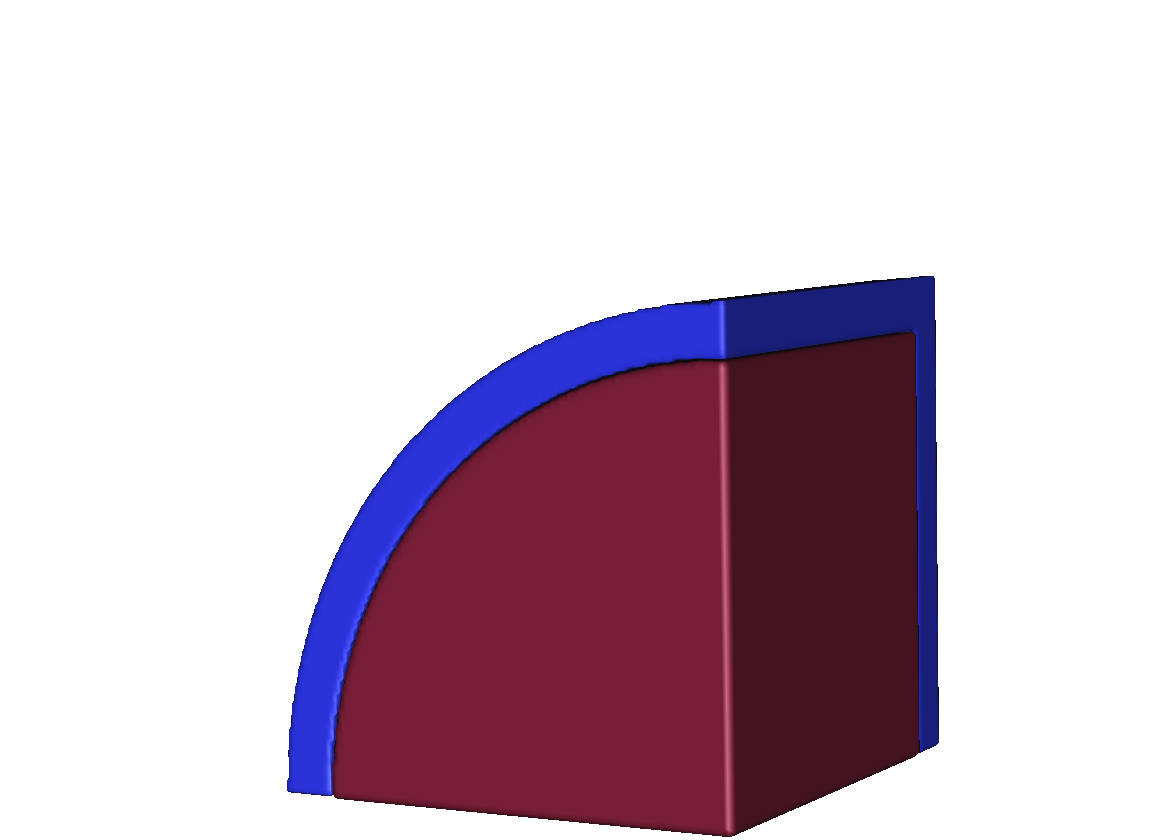
\includegraphics[width=\textwidth]{Figs/mpmice/NE_0_d.png}
   \caption{t=0 $ms$}
   \label{figCookoff:a}
 \end{subfigure}
 \begin{subfigure}[b]{0.3\textwidth}
   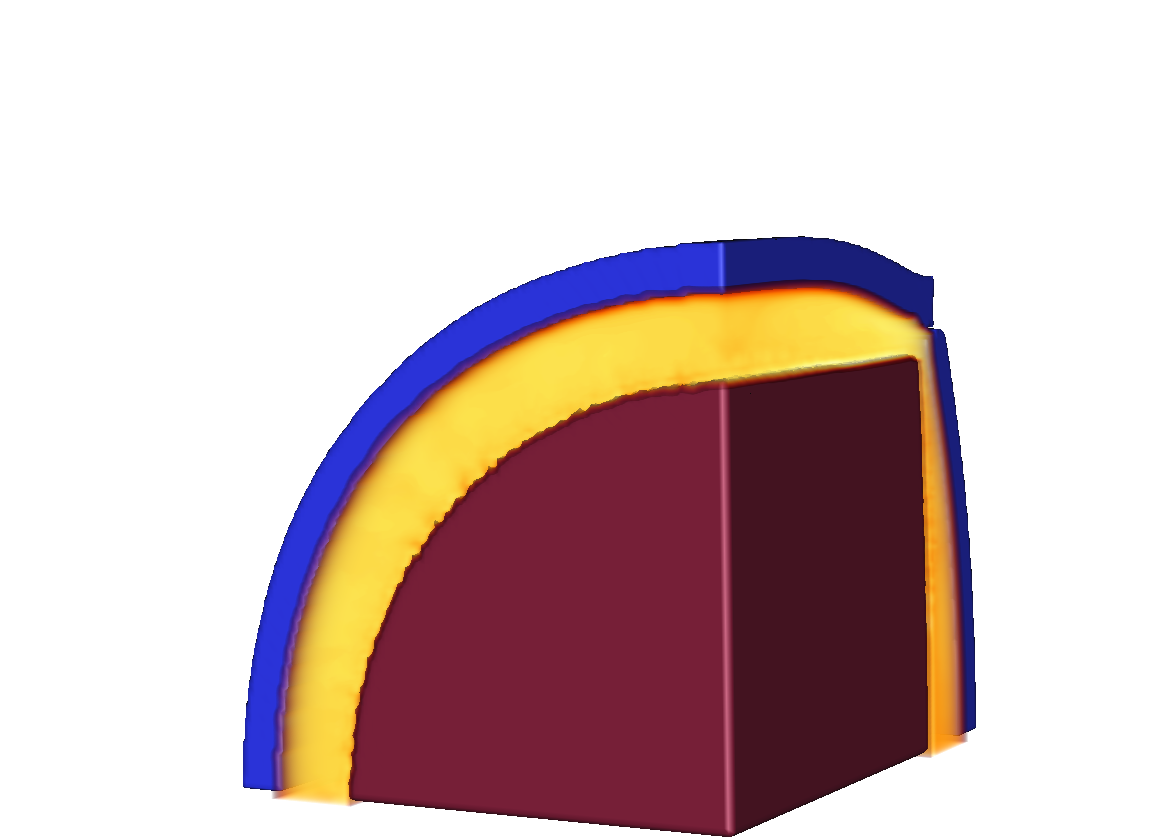
\includegraphics[width=\textwidth]{Figs/mpmice/NE_46_c.png}
   \caption{t=.137 $ms$}
   \label{figCookoff:b}
 \end{subfigure}
 \begin{subfigure}[b]{0.3\textwidth}
   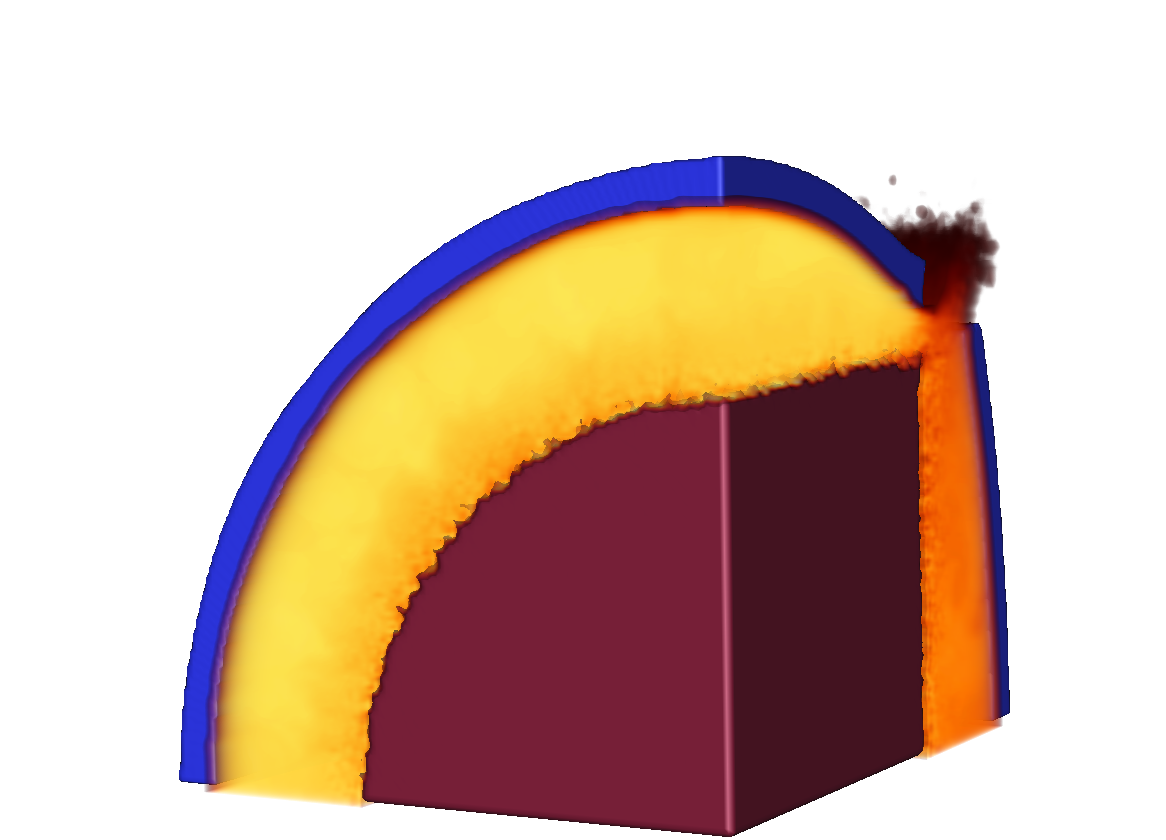
\includegraphics[width=\textwidth]{Figs/mpmice/NE_98_c.png}
   \caption{t=.203 $ms$}
   \label{figCookoff:c}
 \end{subfigure}
 \begin{subfigure}[b]{0.3\textwidth}
   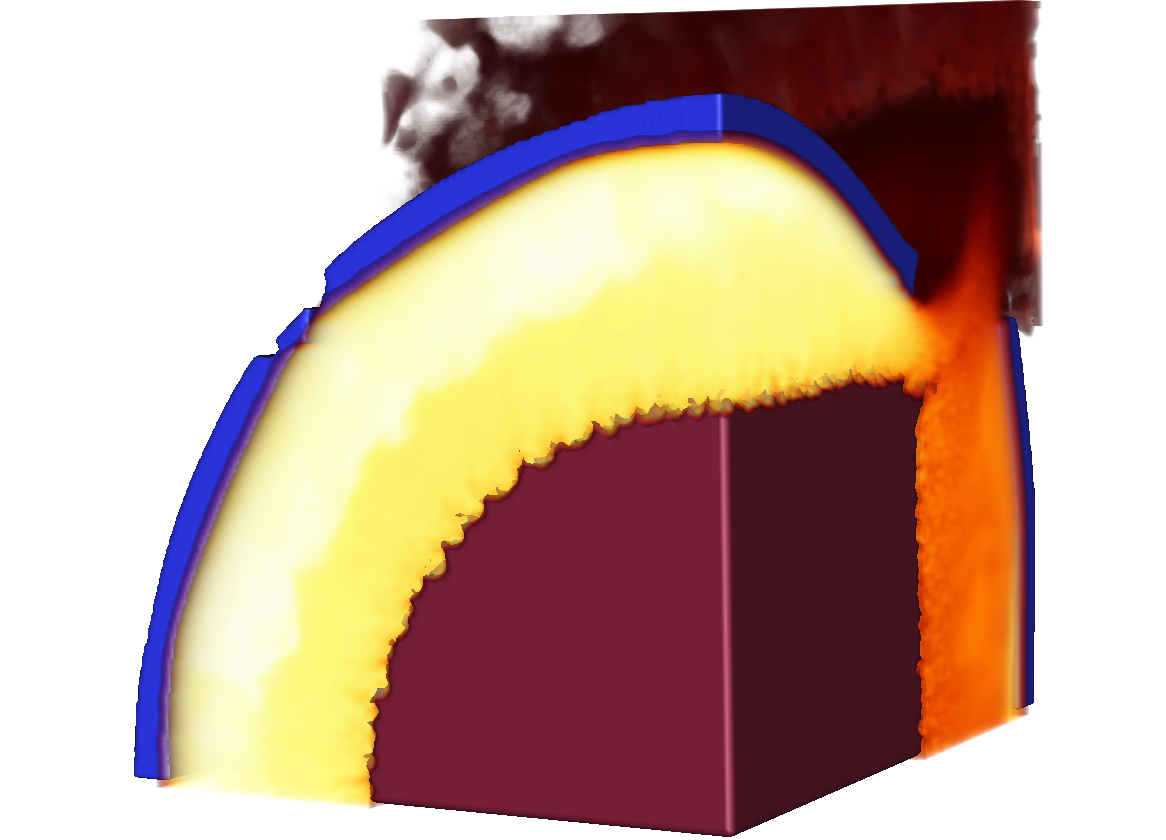
\includegraphics[width=\textwidth]{Figs/mpmice/NE_129_c.png}
   \caption{t=.259 $ms$}
   \label{figCookoff:d}
 \end{subfigure}
 \begin{subfigure}[b]{0.3\textwidth}
   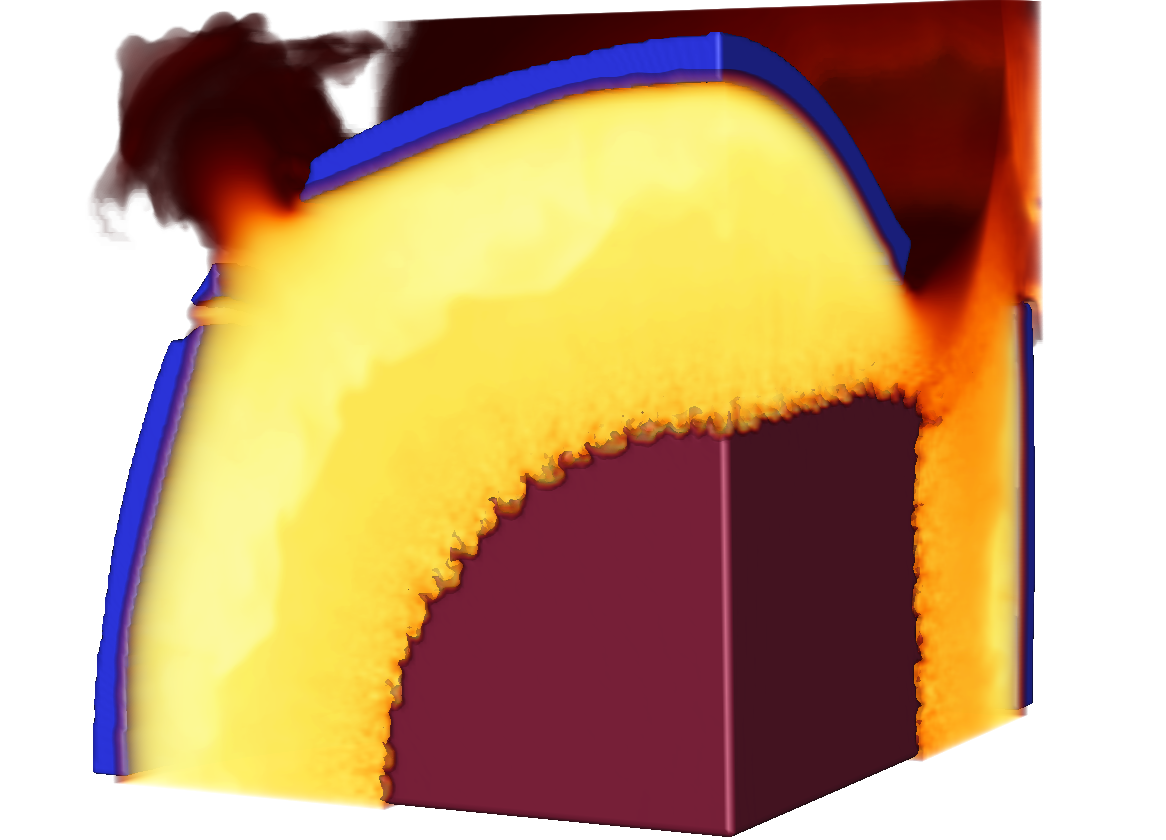
\includegraphics[width=\textwidth]{Figs/mpmice/NE_172_c.png}
   \caption{t=.312 $ms$}
   \label{figCookoff:e}
 \end{subfigure}
 \begin{subfigure}[b]{0.3\textwidth}
   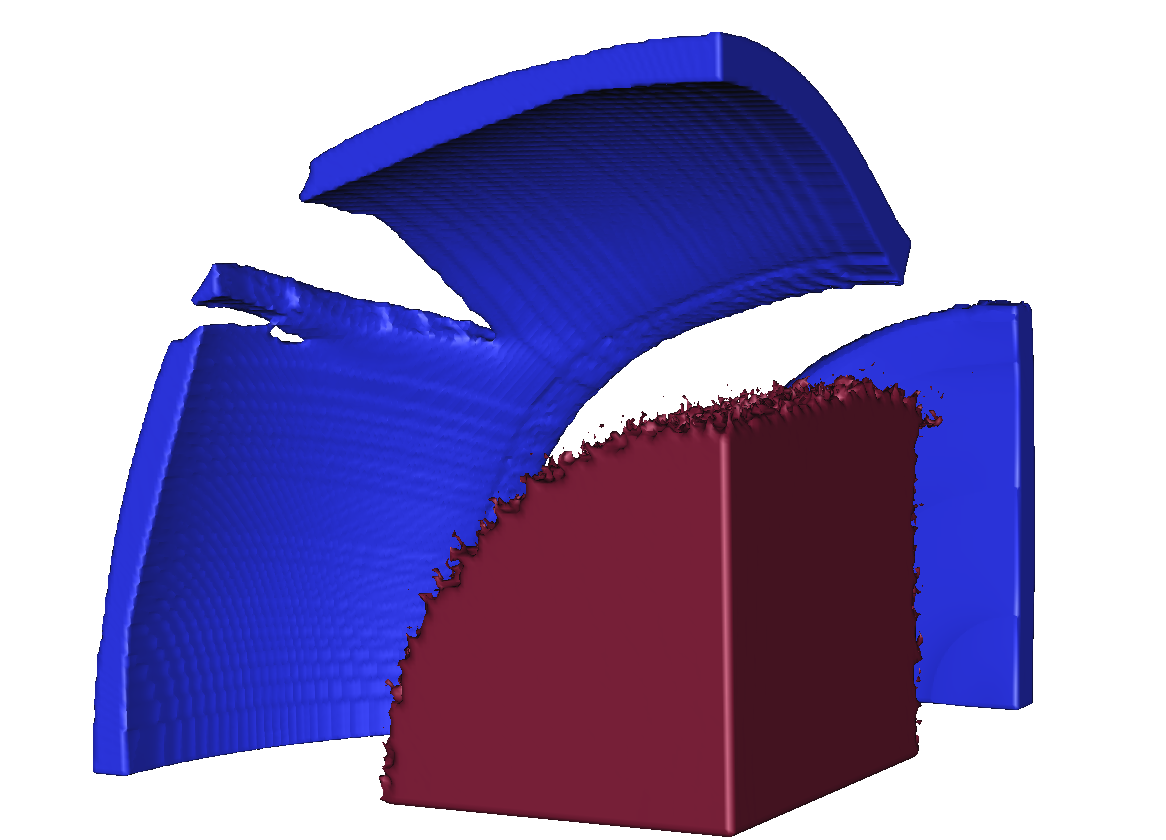
\includegraphics[width=\textwidth]{Figs/mpmice/NE_172_d.png}
   \caption{t=.312 $ms$}
   \label{figCookoff:f}
 \end{subfigure}
 \caption{Time series of a steel container (blue) filled with deflagrating 
          plastic bonded explosive(red).  A volume rendering of the mass 
          density of the products of reaction is also shown, except in the 
          final panel, where it is removed to more clearly show the regions 
          where the container has failed. }
 \label{figCookoff}
 \end{figure}

Since no surface tracking is required in this method, there is no
requirement to track the creation of the new surfaces that occur
due to material failure.  Gas is free to escape through the openings
simply because there is no longer anything in those computational
cells to prevent it once the gap is sufficiently wide.

\section{Conclusions} 

An approach for solving full-physics fluid-structure interaction scenarios 
has been presented which uses a Eulerian frame description for fluids and 
a Lagrangian frame description for solids.  The equations governing the 
behavior of these materials, including their interactions, are based on an 
averaged model approach, which eliminates the need to maintain a description 
of the interface between the materials.  In addition to allowing for 
arbitrary distortion of material interfaces, the treatment of solid to gas 
phase reactions is also facilitated by this approach.

The validation calculations presented here give a high degree of confidence
in the quality of the solutions obtained by this method, while the final 
demonstration calculation indicates the complexity of the situations that 
can be considered.  It is important to point out, however, that in the 
authors' experience, this approach is best suited to high deformation rate
problems, and may do less well in situations where the solid is loaded more 
slowly.  This is true for two reasons.  First, while making the algorithm 
implicit in time with respect to pressure is relatively straightforward, doing 
so with respect to the stress waves in the solid is less so.  Implicit 
versions of MPM have been implemented with success, but the strategy for 
incorporating any of these within the integrated formulation is not 
obvious, and may require making the entire algorithm fully implicit in 
time.  Second, as a method for solid mechanics, currently MPM is best suited 
for highly dynamic loading, although improvements are continuously being made
that should improve its performance in quasi-static scenarios.

In order to improve the efficiency of calculations, a structured adaptive mesh 
refinement (SAMR) strategy is being pursued that will allow resources to be 
concentrated on those parts of the domain where they are needed.  The current 
implementation allows for the solid materials described using MPM to be 
advanced at a single level of resolution, while those materials integrated
in the Eulerian frame are advanced on an arbitrary number of levels of 
resolution.  Thus, in the final simulation shown here, the container and 
solid explosive, which require the greatest degree of resolution to accurately 
compute the phase transformation and material response, can be represented on 
the finest level.  Meanwhile the region away from the device can advance at a 
lower spatial resolution until container expansion and rupture dictate the need 
for refinement.  This strategy enhances the range of simulations that can be 
considered, reduces the required computational time and lowers the requirement 
for the storage of data.
